\documentclass[11pt]{article}

\usepackage[margin=1in]{geometry}
\usepackage[T1]{fontenc}
\usepackage{lmodern}
\usepackage{listings}
\usepackage[hidelinks]{hyperref}
% Shared, editable vector-figure styles. No shell escape or external assets.
\usepackage{tikz}
\usetikzlibrary{arrows.meta,calc,positioning}
\definecolor{figink}{HTML}{253440}
\definecolor{figgray}{HTML}{667784}
\definecolor{figbluefill}{HTML}{EDF2F6}
\definecolor{figteal}{HTML}{087F83}
\definecolor{figtealfill}{HTML}{E9F5F3}
\definecolor{figred}{HTML}{B82D37}
\definecolor{figredfill}{HTML}{FDEBED}
\definecolor{figorange}{HTML}{AD5800}
\definecolor{figorangefill}{HTML}{FFF2DF}
\definecolor{figgreen}{HTML}{237A46}
\definecolor{figgreenfill}{HTML}{EAF5EC}
\tikzset{
  figarrow/.style={-{Latex[length=2.4mm,width=1.7mm]},line width=.9pt},
  figbox/.style={draw=figgray,fill=figbluefill,rounded corners=2pt,
    align=center,inner sep=6pt,line width=.65pt},
  figtrusted/.style={figbox,draw=figteal,fill=figtealfill},
  figlabel/.style={fill=white,inner sep=3pt,align=center},
  fignote/.style={align=center,font=\footnotesize,text=figgray}
}


\lstset{
  basicstyle=\small\ttfamily,
  breaklines=true,
  columns=fullflexible,
  keepspaces=true,
  frame=single,
  showstringspaces=false
}

\title{Decision-Bound Verification for Concurrent A2A Agents: Characterizing TOCTOU Failures and Evaluating Semantic Revalidation}
\author{Project Team}
\date{Draft --- November 8, 2026}

\begin{document}
\maketitle

\begin{abstract}

The Agent2Agent (A2A) protocol enables autonomous agents to collaborate through
asynchronous, multi-turn interactions. However, concurrent agents may modify shared task
state between the time another agent reads information, makes a decision, and executes
an action, introducing time-of-check-to-time-of-use (TOCTOU) vulnerabilities. Recent
work, A2ABreak, identifies this weakness at the protocol level, but its manifestation in
executable multi-agent workflows and the effectiveness of practical interventions remain
insufficiently characterized.

We investigate TOCTOU vulnerabilities in A2A systems through two planned contributions.
First, we plan to develop a reproducible evaluation framework spanning minimal protocol-level races and
realistic multi-agent workflows involving shared resources, delayed decisions, and
concurrent updates. Second, we propose a semantic revalidation mechanism in which agents
generate explicit decision preconditions, an independent LLM verifier checks their
continued validity, and a trusted execution layer enforces the resulting decision using
dependency-aware concurrency control and atomic commits.

We plan experiments comparing our approach against unprotected execution,
coarse-grained locking, task-wide versioning, and conventional dependency-based
revalidation. We will evaluate both security and utility through unsafe-action rates,
legitimate-work preservation, and computational overhead.

Our objective is to characterize when stale decisions produce security failures and
determine whether semantic verification can preserve decision integrity without
unnecessarily restricting parallel agent execution.

\end{abstract}

\section{Introduction}

Autonomous agents are increasingly deployed as collaborative systems rather than
isolated models. Instead of independently completing tasks, agents delegate subtasks,
exchange information, access shared resources, and coordinate across organizational
boundaries. Google's Agent2Agent (A2A) protocol standardizes such interactions,
providing mechanisms for agent discovery, task delegation, asynchronous execution, and
multi-turn communication \cite{a2a-spec}.

However, the ability of agents to operate asynchronously introduces a fundamental
security problem: \textbf{the state upon which an agent makes a decision may no longer
be valid when that decision is acted upon}.

Consider an agent that receives a request to approve a transaction. Before responding,
it reads the transaction amount, recipient, and applicable authorization policy. While
the agent is evaluating the request, another agent modifies the shared task or its
underlying resources. If the first agent subsequently submits its approval without
revalidating the relevant information, the approval may be applied to a transaction
materially different from the one originally evaluated.

Figure~\ref{fig:toctou-attack} illustrates how an honest response can become
stale even when the task identifier and lifecycle status remain unchanged.

\begin{figure}[tbp]
  \centering
  \resizebox{\linewidth}{!}{% Sequence follows the Figure 1 brief; S1/S2 are illustrative labels only.
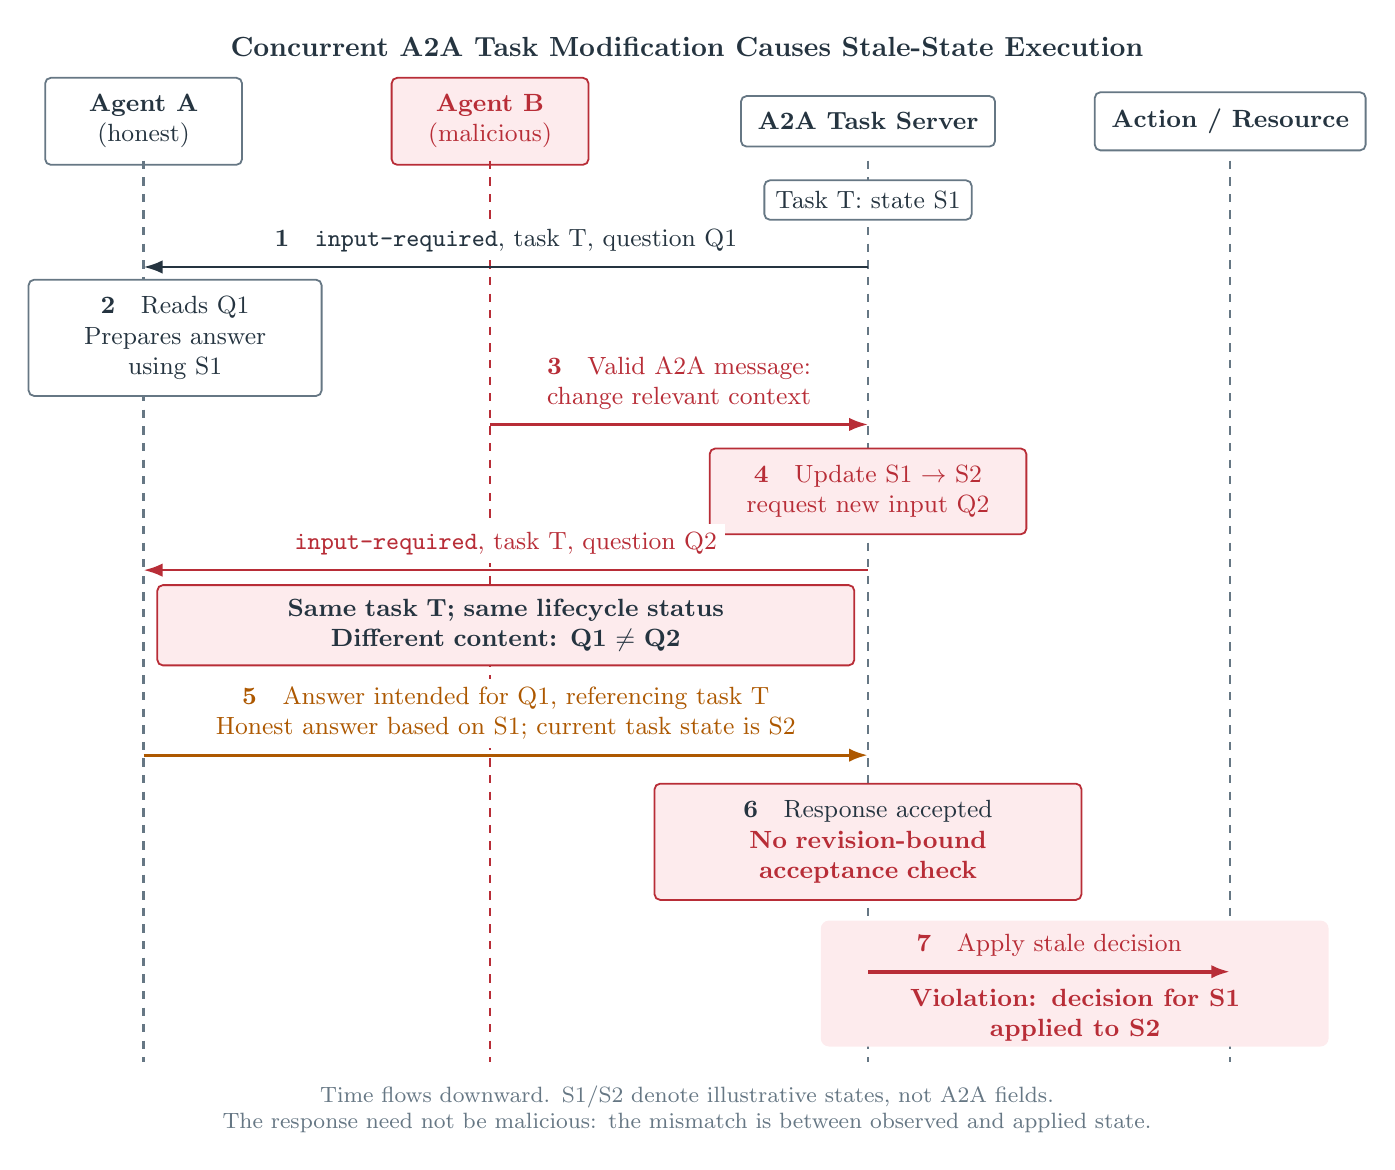
\begin{tikzpicture}[x=1cm,y=1cm,font=\fontsize{9}{11}\selectfont,text=figink]
  \node[font=\bfseries] at (8.15,.95)
    {Concurrent A2A Task Modification Causes Stale-State Execution};
  \node[figbox,fill=white,minimum width=2.5cm] at (1.25,0)
    {\textbf{Agent A}\\(honest)};
  \node[figbox,draw=figred,fill=figredfill,text=figred,minimum width=2.5cm]
    at (5.65,0) {\textbf{Agent B}\\(malicious)};
  \node[figbox,fill=white,minimum width=2.6cm] at (10.45,0)
    {\textbf{A2A Task Server}};
  \node[figbox,fill=white,minimum width=2.6cm] at (15.05,0)
    {\textbf{Action / Resource}};
  \foreach \x in {1.25,10.45,15.05}
    \draw[dashed,figgray,line width=.8pt] (\x,-.5)--(\x,-11.95);
  \draw[dashed,figred,line width=.8pt] (5.65,-.5)--(5.65,-11.95);

  \node[figbox,fill=white,inner sep=4pt] at (10.45,-1)
    {Task T: state S1};
  \draw[figarrow,figink] (10.45,-1.85)--(1.25,-1.85)
    node[midway,figlabel,above=2pt]
    {\textbf{1}\quad \texttt{input-required}, task T, question Q1};
  \node[figbox,text width=3.3cm,fill=white] at (1.65,-2.75)
    {\textbf{2}\quad Reads Q1\\Prepares answer\\using S1};

  \draw[figarrow,figred] (5.65,-3.85)--(10.45,-3.85)
    node[midway,figlabel,above=2pt,text=figred,text width=4.1cm]
    {\textbf{3}\quad Valid A2A message:\\change relevant context};
  \node[figbox,draw=figred,fill=figredfill,text=figred,text width=3.6cm]
    at (10.45,-4.7) {\textbf{4}\quad Update S1 $\rightarrow$ S2\\request new input Q2};
  \draw[figarrow,figred] (10.45,-5.7)--(1.25,-5.7)
    node[midway,figlabel,above=2pt,text=figred]
    {\texttt{input-required}, task T, question Q2};
  \node[figbox,draw=figred,fill=figredfill,inner sep=5pt,text width=8.5cm]
    at (5.85,-6.4)
    {\textbf{Same task T; same lifecycle status}\\\textbf{Different content: Q1 $\ne$ Q2}};

  \draw[figarrow,figorange,line width=1.2pt] (1.25,-8.05)--(10.45,-8.05)
    node[midway,figlabel,above=2pt,text=figorange,text width=8.5cm]
    {\textbf{5}\quad Answer intended for Q1, referencing task T\\
      Honest answer based on S1; current task state is S2};
  \node[figbox,draw=figred,fill=figredfill,text width=5cm]
    at (10.45,-9.15)
    {\textbf{6}\quad Response accepted\\
      \textcolor{figred}{\textbf{No revision-bound acceptance check}}};

  \fill[figredfill,rounded corners=3pt] (9.85,-10.15) rectangle (16.3,-11.75);
  \draw[figarrow,figred,line width=1.3pt] (10.45,-10.8)--(15.05,-10.8)
    node[midway,figlabel,fill=figredfill,above=2pt,text=figred]
    {\textbf{7}\quad Apply stale decision};
  \node[text=figred,font=\fontsize{9}{11}\selectfont\bfseries,align=center,text width=6cm] at (13.08,-11.35)
    {Violation: decision for S1\\applied to S2};
  \node[fignote,text width=15.7cm] at (8.15,-12.55)
    {Time flows downward. S1/S2 denote illustrative states, not A2A fields.\\
      The response need not be malicious: the mismatch is between observed and applied state.};
\end{tikzpicture}
}
  \caption{A protocol-compliant concurrent update changes the conditions
    of an ongoing A2A task after Agent A observes its state. Without
    revision-bound validation, A's subsequent response may be processed
    against a different task state from the one it evaluated. S1/S2 are
    illustrative state labels, not fields supplied by A2A.}
  \label{fig:toctou-attack}
\end{figure}

This is a time-of-check-to-time-of-use (TOCTOU) vulnerability. Although TOCTOU is well
established in conventional computer systems, its manifestation in LLM-agent workflows
introduces additional challenges. Agent decisions can involve extended reasoning,
delayed tool execution, human intervention, and multiple independently evolving sources
of information. Furthermore, the conditions underlying an agent's decision are
frequently expressed in natural language, rather than predefined programmatic
predicates.

Lotfi et al. \cite{a2abreak} identify \textbf{Concurrent Access TOCTOU} as one of eleven
vulnerabilities in the A2A protocol. Their specification-level analysis demonstrates
that the absence of a standardized task-state versioning mechanism permits stale-state
decisions under concurrent access. However, the study primarily establishes the
protocol-level vulnerability rather than experimentally characterizing its behavior
across executable A2A workflows or evaluating alternative runtime defenses.

A straightforward intervention is to lock shared task state or invalidate decisions
whenever the task changes. Although conservative concurrency control can prevent
stale-state races, it may unnecessarily interfere with legitimate parallel execution.
For instance, a change to an unrelated progress message should not necessarily
invalidate an approval based on a transaction's price and recipient.

This motivates a more selective approach: \textbf{rather than treating every state
change as a security-relevant conflict, determine whether the change invalidates the
conditions that justified the original decision}.

We investigate this problem through a two-part study. First, we plan to construct
reproducible A2A environments that expose TOCTOU failures under controlled concurrent interactions.
Second, we propose a verifier-assisted mechanism that represents agent decisions through
explicit acceptance criteria, independently validates those criteria against current
task state, and binds successful verification to the eventual execution through atomic
enforcement.

Our central research question is:

\emph{Can semantic verification of agent decisions prevent TOCTOU vulnerabilities in
concurrent A2A workflows while preserving more legitimate parallel execution than
conventional task-wide concurrency controls?}

\subsection{Motivation}

Existing concurrency mechanisms provide strong foundations for detecting and preventing
stale-state updates. However, long-running agent workflows make the distinction between
a \textbf{state change} and a \textbf{decision-invalidating change} particularly
important.

For example, consider an agent approving a purchase conditional on the vendor's
authorization status and the presence of a valid warranty. Another agent may modify a
vendor document while approval is pending. A minor formatting update should not
invalidate the purchase, whereas a change indicating that the vendor is no longer
authorized should.

These updates may occur outside the structured fields of the original approval request.
Consequently, a fixed set of monitored fields may miss relevant dependencies, while
task-wide locking or versioning may unnecessarily reject independent work.

We are interested in whether an LLM-based verifier can identify these semantic
dependencies, including dependencies that were not explicitly programmed beforehand, and
whether such verification can be integrated with deterministic concurrency enforcement.

The challenge is not merely detecting suspicious modifications. It is preserving the
relationship between the \textbf{evidence an agent observed}, the \textbf{conditions
justifying its decision}, and the \textbf{state against which that decision is
executed}.

\subsection{Theory of Change}

The security of multi-agent systems depends not only on the behavior of individual
agents, but also on the integrity of decisions across interactions with a changing
environment. Even well-behaved agents can produce unsafe outcomes when their decisions
are executed against stale state.

We hypothesize that expressing agent decisions as independently verifiable conditions
can improve the security and efficiency of concurrent agent workflows. By separating
semantic decision validation from deterministic state enforcement, a system may identify
which concurrent modifications genuinely invalidate a decision without blocking
unrelated work.

Our proposed approach operates at three conceptual levels. First, agents expose the
acceptance criteria underlying consequential decisions. Second, an independent verifier
examines whether those criteria are sufficient and remain satisfied by authoritative
task state. Third, a trusted execution mechanism ensures that verification and the
corresponding committed action are consistent, rejecting or revalidating operations when
relevant state changes.

Figure~\ref{fig:verification-architecture} distinguishes agent computation,
independent verification, and atomic enforcement. The commit boundary is
proposed application logic, not an existing A2A protocol guarantee.

\begin{figure}[tbp]
  \centering
  \resizebox{\linewidth}{!}{% Conceptual proposal: version tokens are supplied by the application/store.
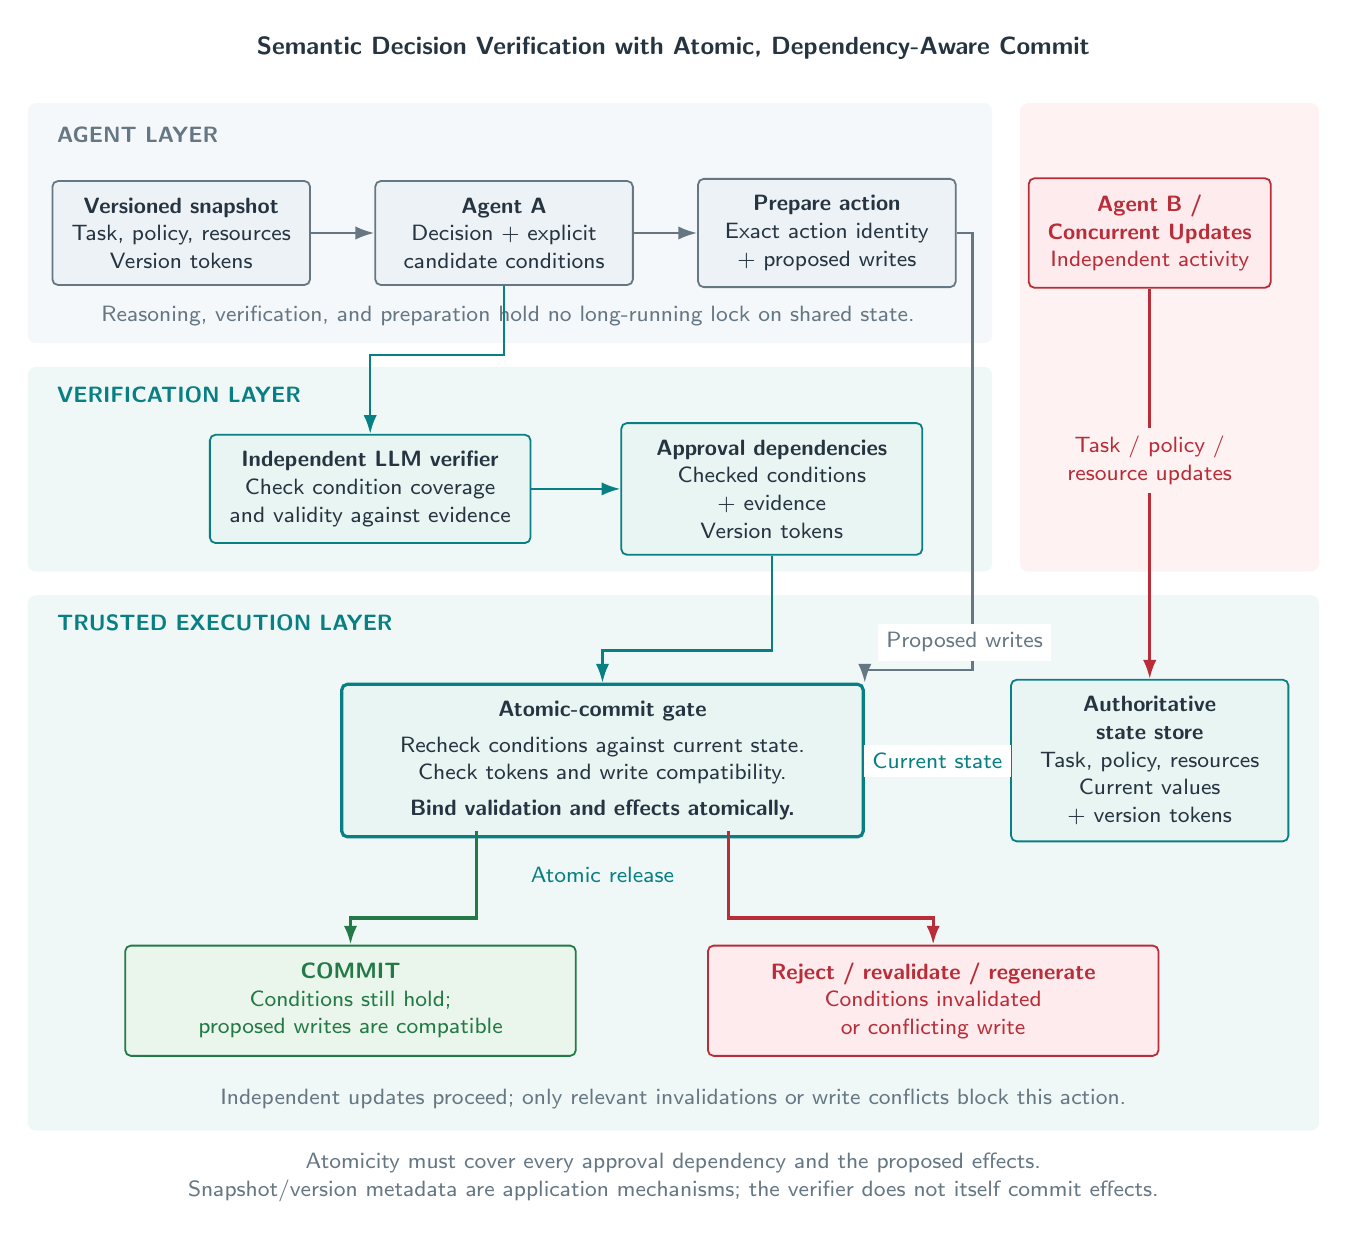
\begin{tikzpicture}[x=1cm,y=1cm,font=\sffamily\fontsize{8}{10}\selectfont,text=figink]
  \node[font=\sffamily\small\bfseries] at (8.2,.85)
    {Semantic Decision Verification with Atomic, Dependency-Aware Commit};
  \fill[figbluefill!55,rounded corners=3pt] (0,.15) rectangle (12.25,-2.9);
  \fill[figtealfill!70,rounded corners=3pt] (0,-3.2) rectangle (12.25,-5.8);
  \fill[figtealfill!70,rounded corners=3pt] (0,-6.1) rectangle (16.4,-12.9);
  \fill[figredfill!65,rounded corners=3pt] (12.6,.15) rectangle (16.4,-5.8);
  \node[anchor=west,font=\sffamily\footnotesize\bfseries,text=figgray]
    at (.25,-.25) {AGENT LAYER};
  \node[anchor=west,font=\sffamily\footnotesize\bfseries,text=figteal]
    at (.25,-3.55) {VERIFICATION LAYER};
  \node[anchor=west,font=\sffamily\footnotesize\bfseries,text=figteal]
    at (.25,-6.45) {TRUSTED EXECUTION LAYER};

  \node[figbox,text width=2.85cm,minimum height=1.25cm] (snapshot) at (1.95,-1.5)
    {\textbf{Versioned snapshot}\\Task, policy, resources\\Version tokens};
  \node[figbox,text width=2.85cm,minimum height=1.25cm] (decision) at (6.05,-1.5)
    {\textbf{Agent A}\\Decision + explicit\\candidate conditions};
  \node[figbox,text width=2.85cm,minimum height=1.25cm] (writes) at (10.15,-1.5)
    {\textbf{Prepare action}\\Exact action identity\\+ proposed writes};
  \draw[figarrow,figgray] (snapshot)--(decision);
  \draw[figarrow,figgray] (decision)--(writes);
  \node[align=center,text=figgray] at (6.1,-2.55)
    {Reasoning, verification, and preparation hold no long-running lock on shared state.};

  \node[figbox,draw=figred,fill=figredfill,text=figred,text width=2.65cm,
    minimum height=1.25cm] (concurrent) at (14.25,-1.5)
    {\textbf{Agent B /}\\\textbf{Concurrent Updates}\\Independent activity};
  \node[figtrusted,text width=3.1cm,minimum height=1.45cm] (store) at (14.25,-8.2)
    {\textbf{Authoritative state store}\\Task, policy, resources\\Current values\\+ version tokens};
  \draw[figarrow,figred,line width=1pt] (concurrent.south)--(store.north)
    node[pos=.44,figlabel,text=figred,text width=2.2cm,fill=figredfill!65]
    {Task / policy /\\resource updates};

  \node[figtrusted,text width=3.65cm,minimum height=1.3cm] (verifier) at (4.35,-4.75)
    {\textbf{Independent LLM verifier}\\Check condition coverage\\and validity against evidence};
  \node[figtrusted,text width=3.4cm,minimum height=1.3cm] (dependencies) at (9.45,-4.75)
    {\textbf{Approval dependencies}\\Checked conditions\\+ evidence\\Version tokens};
  \draw[figarrow,figteal] (decision.south)--(6.05,-3.05)-|(verifier.north);
  \draw[figarrow,figteal] (verifier)--(dependencies);

  \node[figtrusted,line width=1.15pt,text width=6.2cm,minimum height=1.8cm]
    (gate) at (7.3,-8.2)
    {\textbf{Atomic-commit gate}\\[3pt]
      Recheck conditions against current state.\\
      Check tokens and write compatibility.\\[3pt]
      \textbf{Bind validation and effects atomically.}};
  \draw[figarrow,figteal] (dependencies.south)--(9.45,-6.8)-|(gate.north);
  \draw[figarrow,figgray] (writes.east)--(12,-1.5)--(12,-7.05)
    -|(gate.north east);
  \node[figlabel,text=figgray] at (11.9,-6.7) {Proposed writes};
  \draw[figarrow,figteal] (store.west)--(gate.east)
    node[midway,figlabel,text=figteal] {Current state};
  \node[align=center,text=figteal] at (7.3,-9.65)
    {Atomic release};

  \node[figbox,draw=figgreen,fill=figgreenfill,text=figgreen,text width=5.3cm,
    minimum height=1.4cm] (commit) at (4.1,-11.25)
    {\textbf{COMMIT}\\Conditions still hold;\\proposed writes are compatible};
  \node[figbox,draw=figred,fill=figredfill,text=figred,text width=5.3cm,
    minimum height=1.4cm] (reject) at (11.5,-11.25)
    {\textbf{Reject / revalidate / regenerate}\\Conditions invalidated\\or conflicting write};
  \draw[figarrow,figgreen,line width=1.2pt] (5.7,-9.1)--(5.7,-10.2)
    -|(commit.north);
  \draw[figarrow,figred,line width=1.2pt] (8.9,-9.1)--(8.9,-10.2)
    -|(reject.north);
  \node[align=center,text=figgray,text width=15.7cm] at (8.2,-12.5)
    {Independent updates proceed; only relevant invalidations or write conflicts block this action.};
  \node[align=center,text=figgray,text width=16cm] at (8.2,-13.5)
    {Atomicity must cover every approval dependency and the proposed effects.\\
      Snapshot/version metadata are application mechanisms; the verifier does not itself commit effects.};
\end{tikzpicture}
}
  \caption{The proposed framework converts agent-generated decision
    conditions into independently checked approval dependencies. Agents
    operate on versioned snapshots without holding long-running locks.
    Before consequential effects are committed, the trusted execution
    layer atomically validates the relevant conditions against current
    state, permitting independent updates while rejecting stale or
    unauthorized actions. This requires atomic enforcement covering the
    relevant dependencies and proposed effects.}
  \label{fig:verification-architecture}
\end{figure}

If successful, this mechanism could provide a reusable foundation for safer A2A
interoperability: agents could continue reasoning and collaborating concurrently, while
consequential actions remain tied to the conditions that authorize them.

Beyond the proposed intervention, reproducible attack environments could help protocol
developers identify where A2A implementations require additional concurrency guarantees
and evaluate alternative solutions under comparable conditions.

\section{Related Work}

\subsection{Agent-to-Agent Protocols and Security}

The Agent2Agent protocol provides a standardized interface for communication among
autonomous agents, including task creation, state tracking, multi-turn exchanges,
streaming updates, and asynchronous execution \cite{a2a-spec}. These capabilities
support distributed workflows in which multiple agents exchange information and operate
over persistent task contexts.

However, protocol-level interoperability does not necessarily guarantee
application-level security. Li et al. \cite{a2asecbench} introduce A2ASecBench, a
protocol-aware evaluation framework covering six attack families across A2A discovery,
orchestration, and execution. Their work demonstrates the importance of evaluating
security alongside legitimate task utility, but does not specifically benchmark
concurrent stale-decision failures.

Lotfi et al. \cite{a2abreak} develop A2ABreak, a systematic security analysis of the A2A
specification using a formally grounded finite-state-machine framework. Among eleven
identified vulnerabilities, their Concurrent Access TOCTOU finding concerns the absence
of task-state versioning and conditional update semantics. Their analysis motivates the
first part of our work: constructing executable environments to characterize stale-state
failures and evaluate their consequences under controlled concurrency.

\subsection{Concurrency Control in Multi-Agent Systems}

Classical concurrency-control mechanisms, including locking and optimistic concurrency
control, provide techniques for coordinating access to shared mutable state. However, AI
agents introduce long-running operations that may interleave model inference, tool
calls, and external interactions, making coarse locking or repeated transaction retries
potentially expensive.

Lyu et al. \cite{coagent} propose CoAgent, a concurrency-control system for multi-agent
workflows that incorporates LLM-based judgments of whether conflicting writes invalidate
an agent's plan. Rather than relying solely on conventional abort-and-retry behavior,
CoAgent supports selective repair of affected operations. This work demonstrates the
potential value of semantic reasoning in agent concurrency control.

Peng and Wu \cite{stateful-governance} investigate stateful governance for concurrent
agentic systems, formalizing correctness requirements for actions whose authorization
depends on mutable policy state. Their work emphasizes that authorization must remain
valid when consequential effects occur, and that concurrency mechanisms should preserve
legitimate parallel execution without permitting stale authorization.

These approaches establish that semantic conflict detection and state-dependent
authorization are important problems. Our work focuses specifically on adversarial
TOCTOU scenarios in A2A communication, with attention to the reliability of
automatically generated decision conditions and their use in independent verification.

\subsection{Decision-Level Revalidation}

Lyu et al. \cite{selective-revalidation} introduce selective revalidation for
long-running AI agents, distinguishing ordinary version conflicts from changes that
invalidate the justification for an agent's decision. Their proposed runtime records
explicit executable preconditions and selectively rechecks affected dependencies before
releasing an operation. Atomic transactions or compare-and-set mechanisms are used to
bind verified state to execution.

This work is particularly close to ours and provides an important conceptual foundation.
However, its prototype relies on developer-specified conditions rather than
automatically extracting decision requirements from agent behavior.

We investigate whether agents can generate their own decision conditions and whether
independent LLM verification can recover omitted or implicit dependencies. We further
situate this problem within A2A-specific concurrent interactions, comparing semantic
revalidation against established consistency mechanisms under both malicious and benign
modifications.

Our contribution is therefore not a replacement for conventional transaction isolation
or atomic enforcement. Rather, we study whether model-based verification can help
determine \textbf{what must remain true} for an agent's prior decision to stay valid,
while trusted concurrency mechanisms guarantee that the relevant checks are enforced at
execution.

\section{Current Project Scope}
An approval such as ``proceed with the purchase'' leaves its assumptions
implicit. A price, vendor authorization, or warranty observed during an
initial read can change before the action is accepted. Our goal is to make
the approval criteria visible and reviewable, so the application can check
whether they still hold.

The initial artifact is an application-level approval system prompt in
\path{prompts/approval_system.txt}, with integration guidance in
\path{docs/approval_workflow.md}. This is a proposed project convention,
not an adopted A2A protocol change. No existing approval-model call site
was identified in this checkout; loading the prompt into the approval
agent remains an integration task. A separate team workstream owns the
test environment under \path{samples/}.

\section{Approval Response}
The protocol's in-task authorization workflow already covers human
approval: delegated authorization uses \texttt{TASK\_STATE\_AUTH\_REQUIRED}
with an explanatory status message. Authorization is returned out of band
unless an in-band mechanism is negotiated. Its scope and validity are
implementation- or extension-defined\footnote{\href{https://a2a-protocol.org/latest/specification/\#76-in-task-authorization}{A2A specification, section 7.6: In-Task Authorization},
accessed November 8, 2026.}.

The reviewer should explain its recommendation with a concise summary of
the evidence and return explicit conditions before acceptance. Conditions
may use plain language or pseudocode. An illustrative purchase review is:

\noindent\begin{minipage}{\linewidth}
\begin{lstlisting}
{
  "decision": "approve",
  "conditions": [
    "total_price_usd <= 600",
    "vendor.authorized == true",
    "warranty.valid == true"
  ],
  "explanation": "The current quote totals 580 USD including all charges; vendor authorization and warranty validity are confirmed for this purchase."
}
\end{lstlisting}
\end{minipage}

\noindent The spending limit and currency are illustrative, not a default
policy. Each actual review
must use the trusted policy and evidence for the exact proposed action.

The allowed decisions are \texttt{approve}, \texttt{reject}, and
\texttt{needs\_information}. Approval requires a nonempty condition list
covering every applicable policy requirement and evidence supporting each
one. A known violation requires rejection. Missing, stale, ambiguous, or
conflicting required evidence requires more information. The explanation
summarizes the decision-relevant facts rather than requesting private
model reasoning.

\section{Read, Review, Accept, and Execute}
The proposed application workflow is:
\begin{enumerate}
  \item Read the proposed action and authoritative evidence. Record the
    action identity, relevant resource versions, and trusted policy.
  \item Ask the approval reviewer for a decision, conditions, and
    explanation. Treat task and vendor content as evidence, not policy.
  \item Validate the response and show the explanation and conditions
    alongside the exact action to the designated acceptance authority.
  \item Before acceptance, check all trusted policy requirements against
    current authoritative data. If execution is delayed, revalidate again
    before executing the accepted action.
  \item Where supported, apply resource-version checks or preconditions
    atomically with execution. Retain the review and acceptance evidence.
\end{enumerate}

An application's \texttt{AgentExecutor.execute} is the intended integration
point. A possible authorization handoff is a message with text and structured
review data passed to \path{TaskUpdater.requires_auth}. Application
logic must obtain authorization through the agreed channel, check its scope,
and perform policy checks. Ordinary follow-up messages do not automatically
constitute authorization.
The prompt artifact alone does not implement this workflow.

A protocol-level extension would additionally define interoperable action
identifiers, condition semantics, authorization validity, and the negotiated
return channel. The initial prompt asset does not implement that extension.

\section{Enforcement Boundary}
A model's \texttt{approve} is a recommendation, not user consent or proof
that the conditions hold. The application must validate the response,
check every trusted requirement independently of the model's list, and
bind acceptance to the exact action. Condition strings are descriptive;
they must not be evaluated as arbitrary code.

Fresh reads reduce reliance on stale evidence but cannot eliminate a race
between a check and an external action. Atomic conditional execution,
transactions, or an equivalent mechanism are needed where available.
Where unavailable, the remaining race must be recorded as a limitation.

\section{Evaluation Plan}
Compare a decision-only baseline with the proposed prompt in the team's
test environment. Include compliant actions, individual policy violations,
missing evidence, contradictory evidence, malformed responses, and task
content that attempts to override the policy. Change the price, vendor
authorization, warranty, or proposal between the initial read, approval,
and execution to test stale decisions and action binding.

Measure response-contract validity, coverage of trusted requirements,
unsupported-approval rate, detection of stale approvals, and additional
approval latency. Separate prompt adherence from application enforcement:
a compliant explanation is not evidence that an action was blocked.
Record the model and prompt versions, policy, trial count, evidence
versions, mutation timing, and execution outcomes for reproducibility.

\section{Implementation Status and Results}
\textbf{Current status:} reusable prompt and integration specification;
report scaffold. Runtime prompt loading, response validation, trusted
policy evaluation, action binding, and acceptance handling are pending.

\textbf{Results:} no approval-model experiment or attack evaluation has
been run for this draft. Add measured outcomes and uncertainty after the
test environment and runtime integration are available.


\begin{thebibliography}{9}

\bibitem{a2a-spec}
A2A Project. \emph{Agent2Agent Protocol Specification}, v1.0.0.
\url{https://a2a-protocol.org/v1.0.0/specification/}

\bibitem{a2abreak}
Lotfi, A., Rahman, M. M., Karim, I., \& Bertino, E. (2026). \emph{A2ABreak: Systematic Security Analysis of the A2A Protocol}. ACSAC 2026.
\url{https://arxiv.org/abs/2609.10871}

\bibitem{a2asecbench}
Li, T., Chu, C., Zheng, Y., Zhang, B., Gong, N. Z., \& Xiao, C. (2026). \emph{A2ASecBench: A Protocol-Aware Security Benchmark for Agent-to-Agent Multi-Agent Systems}. ICLR 2026.
\url{https://openreview.net/forum?id=LfdFnakqGJ}

\bibitem{coagent}
Lyu, H., Zhang, D., Wu, M., Wei, X., \& Chen, H. (2026). \emph{CoAgent: Concurrency Control for Multi-Agent Systems}.
\url{https://arxiv.org/abs/2606.15376}

\bibitem{stateful-governance}
Peng, Y., \& Wu, X. (2026). \emph{Stateful Governance for Concurrent Agentic Systems}.
\url{https://arxiv.org/abs/2608.02764}

\bibitem{selective-revalidation}
Lyu, Y., Ren, Y., Lai, R., \& Liu, W. (2026). \emph{From Version Conflicts to Decision Conflicts: Selective Revalidation for Long-Running AI Agents}.
\url{https://arxiv.org/abs/2609.08015}

\end{thebibliography}

\end{document}
